\documentclass[utf8, russian, hpadding=5mm, vpadding=15mm, floatsection, columnxxvi, columnxxxi, columnxxxii, equationsection, pointsection, footnoteasterisk]{eskdtext}

%доп. пакеты
\usepackage{amsfonts, amsmath, amssymb}	%Для математических штуковин
\usepackage{wallpaper}					%Для вставки сторонних страниц		
\usepackage{multirow}
%доп. настройки
\bibliographystyle{ugost2008}					%Стиль списка литературы
\graphicspath{{./images/}{./extrapdfpages/}}	%Папки с картинками

%на случай, если команда не определена
\newcommand{\No}{\textnumero}

%для определения форматирования нумерации элементов списка литературы
\makeatletter
\renewcommand{\@biblabel}[1]{#1}
\makeatother

%для штампа	
\ESKDtitle{{\small РИРМ “Интеллектуальное управление в условиях неопределенности”}\\ \small Пояснительная записка}
\ESKDsignature{КСУИ.06.4135.001 ПЗ}
\ESKDgroup{\footnotesize Университет ИТМО\\Кафедра СУиИ\\гр.~P4135}
\ESKDauthor{\resizebox{2.22cm}{\height}{Артемов К.}}
\ESKDchecker{\resizebox{2.22cm}{\height}{Ушаков А.В.}}
%\ESKDnormContr{\resizebox{2.22cm}{\height}{ }}
%\ESKDapprovedBy{\resizebox{2.22cm}{\height}{ }}

%оступы от заголовков разделов и подразделов
\ESKDsectSkip{section}{7mm}{7mm}
\ESKDsectSkip{subsection}{5mm}{5mm}
\ESKDsectSkip{subsubsection}{3mm}{3mm}
\renewcommand{\theenumi}{\arabic{enumi}}

%тело документа
\begin{document}
%\addtocounter{page}{1} %если в документ будут вставлены иные страницы (ТЗ и проч.)
\ESKDthisStyle{empty}
\mbox{}
\ThisLRCornerWallPaper{1}{title_page_1.pdf}
\newpage
%\ESKDthisStyle{empty}
%\mbox{}
%\ThisLRCornerWallPaper{1}{title_page2.pdf}
%\newpage

\ESKDthisStyle{formII}
\tableofcontents
\newpage
\topmargin = 0 mm
%4.1 Введение.Постановка задачи								
%4.2.Построение МТЧ НОУи результаты ее исследования	________________________
%4.3.Построение МТЧ ДОУи и результаты ее исследования	________________________
%4.4.Построение МТЧ СНС и результаты ее исследования	________________________
%4.5.Построение МФМЧ и результаты ее исследования__________________		
%4.6.Построение медианного МУ НОУ и оценка его результатов______________________
%4.7.Синтез неадаптивного и адаптивного управления, обеспечивающего параметрическую инвариантность выхода СНС относительно неопределенности НОУ

\section*{Введение. Постановка задачи}
\addcontentsline{toc}{section}{Введение.Постановка задачи}

Задан непрерывный объект управления (НОУ) с помощью передаточной функции (ПФ) «вход-выход (ВВ)»
\begin{equation}\label{eq_pf0}
	\Phi (s, q) = \cfrac{b_0 (1 + q_1) s + b_1 (1 + q_2)}{(a_0 (1+q_3)s + a_1 (1+q_4))(a_2 (1+q_5) s^2 + a_3 (1 + q_6) s + a_4 (1 + q_7))}
\end{equation}
где $q_{10}=q_{20}=q_{30}=q_{40}=q_{50}=q_{60}=q_{70}=0$~--- номинальные значения параметров $q_{j0}, j = \overline{1,7}$.

Необходимо проделать работу в соответствии с заданием на расчетно-исследовательскую  работу магистранта (РИРМ). Исходные данные для варианта~№6 ААББАААА указаны в таблице~\ref{problem_data}.

\begin{table}[h!]
	\caption{Исходные данные}
	\begin{tabular}{|p{0.5\linewidth}|p{0.4\linewidth}|}
%\hline
%Параметр & Значения \\
\hline
1.1. Значения параметров ПФ & 
$b_0 = 3; b_1 = 0.4; a_0=2; a_1 = 0.6; a_2 = 0; a_3 = 6; a_4 = 10$
\\
\hline
1.2. Базис описания НОУ & канонический управляемый
\\
\hline
2.1. Интервал дискретности & $\Delta{t} = 0.03$с\\
\hline
2.2. Метод перехода к ДОУ & с помощью интегральной модели ВСВ НОУ
\\
\hline
3. Характеристическая частота  & $\omega_0 = 3 c^{-1}$\\
\hline
5. Граничные (угловые) значения параметра $q_j$  & $\underline{q_j} = -0.2; \overline{q_j} = 0.2$ \\ 
\hline
6. Относительная интервальность матрицы состояния системы & $\delta_{IR} F = 0.02$\\
\hline
7. Величина параметрической неопределенности  & $\underline{q_j} = -0.2; \overline{q_j} = 0.2$\\
\hline
	\end{tabular}
	\label{problem_data}
\end{table}


\newpage
\section{Построение МТЧ НОУ и результаты ее исследования}\label{problem_1}

\begin{enumerate}
	\item Записать непрерывный ОУ (НОУ) в форме <<вход-состояние-выход (ВСВ)>> в требуемом базисе;
	\item Построить модель траекторной чувствительности (МТЧ) НОУ;
	\item Произвести ранжирование параметров  по потенциальной чувствительности к ним выхода ОУ с использованием матрицы управляемости агрегированной системы; 
	
	Оценить, какое из дополнительных движений, вызванных вариацией, потребует максимальных затрат управления при обеспечении его асимптотической сходимости к нулю.
\end{enumerate}


\subsection{Непрерывный ОУ в форме ВСВ}

Заданный ОУ описывается ПФ
\begin{equation}\label{eq_OU}
\Phi (s, q) = \cfrac{3 (1 + q_1) s + 0.4 (1 + q_2)}{(2 (1+q_3)s + 0.6 (1+q_4))(6 (1 + q_6) s + 10 (1 + q_7))}
\end{equation}

Для составления векторно-матричного описания ОУ запишем ПФ в форме
\begin{equation*}\label{eq_pf_coc}
\Phi (s, q) = \cfrac{\cfrac{(1 + q_1)}{4(1+q_3)(1+q_6)} s + \cfrac{(1 + q_2)}{30(1+q_3)(1+q_6)}}{s^2 + \cfrac{20(1+q_3)(1+q_7)+3.6(1+q_4)(1+q_6)}{12(1+q_3)(1+q_6)} s + \cfrac{(1+q_4)(1+q_7)}{2(1+q_3)(1+q_6)}}
\end{equation*}

В каноническом управляемом базисе векторно-матричное представление ОУ принимает вид:
\begin{equation}\label{eq_iso_coc}
\begin{cases}
\dot x(t,q) &= A(q) x(t,q) + B u(t)\\
y(t,q) &= C(q) x(t,q)
\end{cases}
\end{equation}
в котором
\begin{equation}
	A(q) =
	\begin{bmatrix}
		0 & 1 \\
		- \cfrac{(1+q_4)(1+q_7)}{2(1+q_3)(1+q_6)} & - \cfrac{20(1+q_3)(1+q_7)+3.6(1+q_4)(1+q_6)}{12(1+q_3)(1+q_6)}
	\end{bmatrix}
\end{equation}
\begin{equation}
	B =
	\begin{bmatrix}
		0\\
		1
	\end{bmatrix}
\end{equation}

\begin{equation}
	C(q) =
	\begin{bmatrix}
	\cfrac{(1 + q_2)}{30(1+q_3)(1+q_6)} & \cfrac{(1 + q_1)}{4(1+q_3)(1+q_6)} 
	\end{bmatrix}
\end{equation}

\subsection{Модель траекторной чувствительности НОУ}

ПФ номинального ОУ, когда параметры $q_{j} = 0, j = \overline{1,7}$, представляет собой
\begin{equation}
	\Phi(s, 0) = \cfrac{\cfrac{1}{4} s + \cfrac{1}{30}}{s^2 + \cfrac{236}{120} s + \cfrac{1}{2}} 
\end{equation}

Матрицы модели ВСВ номинального ОУ имеют реализации
\begin{align*}
A =
\begin{bmatrix}
0 & 1 \\
- \cfrac{1}{2} & - \cfrac{236}{120}
\end{bmatrix};
B =
\begin{bmatrix}
0\\
1
\end{bmatrix};
C =
\begin{bmatrix}
\cfrac{1}{30} & \cfrac{1}{4}
\end{bmatrix}
\end{align*}

Введем обозначения
\begin{align*}
	&A_{q_j} = \cfrac{\partial{A(q)}}{\partial{q_j}} \bigg|_{q=q_0};
	B_{q_j} = \cfrac{\partial{B(q)}}{\partial{q_j}} \bigg|_{q=q_0};
	C_{q_j} = \cfrac{\partial{C(q)}}{\partial{q_j}} \bigg|_{q=q_0};\\
	&A(q)|_{q=q_0} = A;
	B(q)|_{q=q_0} = B;
	C(q)|_{q=q_0} = C;\\
	&x(t,q)|_{q=q_0} = x(t);
	y(t,q)|_{q=q_0} = y(t);\\
	&\cfrac{\partial{x(t,q)}}{\partial{q_j}} \bigg|_{q=q_0} = \sigma_j(t);
	\cfrac{\partial{y(t,q)}}{\partial{q_j}} \bigg|_{q=q_0} = \eta_j(t);
\end{align*}

Теперь для $j$-й модели траекторной чувствительности получим представление МТЧ
\begin{equation}\label{eq_mts}
	\begin{cases}
		\dot \sigma_j(t) &= A \sigma_j(t) + A_{q_j} x(t) + B_{q_j} u(t); 
		\sigma_j (0) = 0\\
		\eta_j (t) &= C \sigma_j (t) + C_{q_j} x(t)
	\end{cases}
\end{equation}

МТЧ будет генерировать функции траекторной чувствительности $\sigma_j (t)$ по состоянию и $\eta_j (t)$ по выходу, если ее дополнить моделью номинального ОУ~\ref{eq_iso_coc}.

На состояние заданного ОУ влияют $p = 6$ (далее, под записью $j = \overline{1, p}$ будет подразумеваться, что $j = 1,2,3,4,6,7$) параметров: $q_1, q_2, q_3, q_4, q_6, q_7$. Вычислим матрицы моделей траекторной чувствительности
\begin{align}
	&A_{q_1} = 
	\begin{bmatrix}
		0 & 1\\
		0 & 0
	\end{bmatrix};
	B_{q_1} = 
	\begin{bmatrix}
		0\\
		1
	\end{bmatrix};
	C_{q_1} = 
	\begin{bmatrix}
		0 & \cfrac{1}{4}
	\end{bmatrix};\\
	&A_{q_2} = 
	\begin{bmatrix}
	0 & 1\\
	0 & 0
	\end{bmatrix};
	B_{q_2} = 
	\begin{bmatrix}
	0\\
	1
	\end{bmatrix};
	C_{q_2} = 
	\begin{bmatrix}
	\cfrac{1}{30} & 0
	\end{bmatrix};\\
	&A_{q_3} = 
	\begin{bmatrix}
	0 & 1\\
	\cfrac{1}{2} & \cfrac{36}{120}
	\end{bmatrix};
	B_{q_3} = 
	\begin{bmatrix}
	0\\
	1
	\end{bmatrix};
	C_{q_3} = 
	\begin{bmatrix}
	- \cfrac{1}{30} & - \cfrac{1}{4}
	\end{bmatrix};\\
	&A_{q_4} = 
	\begin{bmatrix}
	0 & 1\\
	- \cfrac{1}{2} & - 3.6
	\end{bmatrix};
	B_{q_4} = 
	\begin{bmatrix}
	0\\
	1
	\end{bmatrix};
	C_{q_4} = 
	\begin{bmatrix}
	0 & 0
	\end{bmatrix};\\
	&A_{q_6} = 
	\begin{bmatrix}
	0 & 1\\
	\cfrac{1}{2} & \cfrac{20}{12}
	\end{bmatrix};
	B_{q_6} = 
	\begin{bmatrix}
	0\\
	1
	\end{bmatrix};
	C_{q_6} = 
	\begin{bmatrix}
	- \cfrac{1}{30} & - \cfrac{1}{4}
	\end{bmatrix};\\
	&A_{q_7} = 
	\begin{bmatrix}
	0 & 1\\
	- \cfrac{1}{2} & - \cfrac{20}{12}
	\end{bmatrix};
	B_{q_7} = 
	\begin{bmatrix}
	0\\
	1
	\end{bmatrix};
	C_{q_7} = 
	\begin{bmatrix}
	0 & 0
	\end{bmatrix};
\end{align}

\subsection{Ранжирование параметров}

Сконструируем агрегированную систему с составным вектором $\tilde{x}_j = col\{x, \sigma_j\}$ размерности $ \dim \tilde{x} = 2n$, которая объединением \ref{eq_mts} и \ref{eq_iso_coc}, получает представление
\begin{align}\label{rang_system}
	\dot{\tilde{x}}_j (t) &= \tilde{A}_j \tilde{x}_j (t) + \tilde{B}_j u(t); 
	\tilde{x}_j (0) = col \{x(0), 0\}\\
	x(t) &= \tilde{C}_{x_j} \tilde{x}_j;\\
	y(t) &= \tilde{C}_j \tilde{x}_j (t);\\
	\sigma_j (t) &= \tilde{C}_{\sigma_j} \tilde{x}_j (t);\\
	\eta_j (t) &= \tilde{C}_{\eta_j} \tilde{x}_j (t)
\end{align}
где 
\begin{align*}
	&j = \overline{1, p},
	\tilde{A}_j =
	\begin{bmatrix}
	A & 0\\
	A_{q_j} & A
	\end{bmatrix},
	\tilde{B}_j = 
	\begin{bmatrix}
		B\\
		B_{q_j}
	\end{bmatrix},\\
	&\tilde{C}_{x_j} = 
	\begin{bmatrix}
		I_{n \times n} & O_{n \times n}
	\end{bmatrix},
	\tilde{C}_{j} = 
	\begin{bmatrix}
		C & 0_{m \times n}
	\end{bmatrix},
	\tilde{C}_{\sigma_{j}} = 
	\begin{bmatrix}
		0_{n \times n} & I_{n \times n}
	\end{bmatrix},
	\tilde{C}_{\eta_{j}} = 
	\begin{bmatrix}
		C_{q_j} & C
	\end{bmatrix}.	
\end{align*}

Составим необходимые матрицы

\begin{align*}
	&\tilde{A}_{1,2} =
	\begin{bmatrix}
		0 & 1 & 0 & 0\\
		- \cfrac{1}{2} & - \cfrac{236}{120} & 0 & 0\\
		0 & 1 & 0 & 1\\
		0 & 0 &- \cfrac{1}{2} & - \cfrac{236}{120}
	\end{bmatrix};
	\tilde{A}_3 =
	\begin{bmatrix}
		0 & 1 & 0 & 0\\
		- \cfrac{1}{2} & - \cfrac{236}{120} & 0 & 0\\
		0 & 1 & 0 & 1\\
		\cfrac{1}{2} & \cfrac{36}{120} &- \cfrac{1}{2} & - \cfrac{236}{120}
	\end{bmatrix};\\
	&\tilde{A}_4 =
	\begin{bmatrix}
		0 & 1 & 0 & 0\\
		- \cfrac{1}{2} & - \cfrac{236}{120} & 0 & 0\\
		0 & 1 & 0 & 1\\
		- \cfrac{1}{2} & - 3.6 &- \cfrac{1}{2} & - \cfrac{236}{120}
	\end{bmatrix};
	\tilde{A}_6 =
	\begin{bmatrix}
		0 & 1 & 0 & 0\\
		- \cfrac{1}{2} & - \cfrac{236}{120} & 0 & 0\\
		0 & 1 & 0 & 1\\
		\cfrac{1}{2} & \cfrac{20}{12} &- \cfrac{1}{2} & - \cfrac{236}{120}
	\end{bmatrix};\\
	&\tilde{A}_7 =
	\begin{bmatrix}
		0 & 1 & 0 & 0\\
		- \cfrac{1}{2} & - \cfrac{236}{120} & 0 & 0\\
		0 & 1 & 0 & 1\\
		- \cfrac{1}{2} & - \cfrac{20}{12} &- \cfrac{1}{2} & - \cfrac{236}{120}
	\end{bmatrix};
	\tilde{B}_{1,2,3,4,6,7} =
	\begin{bmatrix}
		0\\
		1\\
		0\\
		1
	\end{bmatrix};
\end{align*}

\begin{align*}
	&\tilde{C}_{x_{1,2,3,4,6,7}} =
	\begin{bmatrix}
		1 & 0 & 0 & 0\\
		0 & 1 & 0 & 0\\
	\end{bmatrix};
	\tilde{C}_{1,2,3,4,6,7} =
	\begin{bmatrix}
		\cfrac{1}{30} & \cfrac{1}{4} & 0 & 0\\
	\end{bmatrix};\\
	&\tilde{C}_{\sigma_{1,2,3,4,6,7}} =
	\begin{bmatrix}
		0 & 0 & 1 & 0\\
		0 & 0 & 0 & 1\\
	\end{bmatrix};\\
	&\tilde{C}_{\eta_1} =
	\begin{bmatrix}
		0 & \cfrac{1}{4} & \cfrac{1}{30} & \cfrac{1}{4}\\
	\end{bmatrix};
	\tilde{C}_{\eta_2} =
	\begin{bmatrix}
		\cfrac{1}{30} & 0 & \cfrac{1}{30} & \cfrac{1}{4}\\
	\end{bmatrix};\\
	&\tilde{C}_{\eta_3} =
	\begin{bmatrix}
		-\cfrac{1}{30} & - \cfrac{1}{4} & \cfrac{1}{30} & \cfrac{1}{4}\\
	\end{bmatrix};
	\tilde{C}_{\eta_4} =
	\begin{bmatrix}
		0 & 0 & \cfrac{1}{30} & \cfrac{1}{4}\\
	\end{bmatrix};\\
	&\tilde{C}_{\eta_6} =
	\begin{bmatrix}
		- \cfrac{1}{30} & - \cfrac{1}{4} & \cfrac{1}{30} & \cfrac{1}{4}\\
	\end{bmatrix};
	\tilde{C}_{\eta_7} =
	\begin{bmatrix}
		0 & 0 & \cfrac{1}{30} & \cfrac{1}{4}\\
	\end{bmatrix};
\end{align*}

Для ранжирования параметров по возможным затратам ресурсов управления для достижения нечувствительности траектории проектируемой системы к этим вариациям проведем анализ
управляемости системы~\ref{rang_system} по ее выходу~$\eta_j$.

Требования к ресурсам управления заметно снижаются, если изначально ограничиться задачей обеспечения траекторной нечувствительности выхода проектируемой системы. На уровне требований к структурным свойствам агрегированной системы~\ref{rang_system} задача сводится к контролю управляемости тройки матриц $(\tilde{C}_{\eta_j}, \tilde{A}_{j}, \tilde{B}_{j})$ и количественной оценке эффекта управления по переменной $\eta_j$ при приложении управления $u(t)$ фиксированной нормы с помощью сингулярных чисел матрицы управляемости
\begin{equation}
	\tilde{W}_{y \eta_j} =
	\begin{bmatrix}
		\tilde{C}_{\eta_j} \tilde{B}_{j} &
		\tilde{C}_{\eta_j} \tilde{A}_{j} \tilde{B}_{j} &
		\tilde{C}_{\eta_j} \tilde{A}_{j}^2 \tilde{B}_{j} &		
		\cdots &
		\tilde{C}_{\eta_j} \tilde{A}_{j}^{2n-1} \tilde{B}_{j}
	\end{bmatrix}
\end{equation}

С учетом $n = 2$, рассчитаем матрицы управляемости $\tilde{W}_{\eta_j}$
\begin{align*}
	&\tilde{W}_{y \eta_{1}} =
	\begin{bmatrix}
		0.5  & - 0.9166667  &  1.4277778 & - 2.120463   
	\end{bmatrix}, 
	\\
	&\tilde{W}_{y \eta_2} =
	\begin{bmatrix}
		0.25 &  - 0.3916667 &   0.5202778 & - 0.5982130  	
	\end{bmatrix}, 
	\\
	&\tilde{W}_{y \eta_3} =
	\begin{bmatrix}
		0   &   0.1083333 & - 0.3505556 &   0.8681759  
	\end{bmatrix}, 
	\\
	&\tilde{W}_{y \eta_4} =
	\begin{bmatrix}
		0.25 & - 1.325    &    3.8808333 & - 9.3064722  
	\end{bmatrix}, 
	\\
	&\tilde{W}_{y \eta_6} =
	\begin{bmatrix}
		0   &   0.45   &    - 1.6488889  &  4.3117963  
	\end{bmatrix}, 
	\\
	&\tilde{W}_{y \eta_7} =
	\begin{bmatrix}
		0.25 & - 0.8416667 &   2.0441667 & - 4.4350093
	\end{bmatrix}
\end{align*}

Вычислим для полученных матриц управляемости сингулярные числа
\begin{align}\label{singul_nums}
	&\alpha\{\tilde{W}_{y \eta_{1}}\} = 2.7613747,
	\alpha\{\tilde{W}_{y \eta_{2}}\} = 0.9189399,\\	
	&\alpha\{\tilde{W}_{y \eta_{3}}\} = 0.9425257,	
	\alpha\{\tilde{W}_{y \eta_{4}}\} = 10.172975,\\		
	&\alpha\{\tilde{W}_{y \eta_{6}}\} = 4.6382024,
	\alpha\{\tilde{W}_{y \eta_{7}}\} = 4.9617363
	\label{singul_nums_end}
\end{align}


%Ранжирование параметров $q_j$ осуществляется по значению сингулярных чисел матриц управляемости. 
%Чем эти числа меньше, тем большими по норме управлениями достигается асимптотическая траекторная нечувствительность компонента yj(t) вектора выхода y(t). Отсюда следует, что асимптотическая сходимость к нулю дополнительного движения будет требовать все меньшего количества затрат при следующем расположении qj : q6, q7, q2, q4, q5.

Ранги матриц $\tilde{W}_{\eta_j}$ равны $rang(\tilde{W}_{\eta_j}) = 1$, что совпадает с размерностью $m = 1$ вектора выхода. Таким образом, выбором закона
управления можно обеспечить сходимость $\lim_{t  \to \infty} \Delta y (t,q_0,\Delta q_j) = 0; j = \overline{1, p}$ с заданным темпом~\cite{NSUsh}. 
Сингулярные числа матриц $\tilde{W}_{\eta_j}$ принимают значения~\ref{singul_nums}--\ref{singul_nums_end}. Проранжируем параметры $q_j$ в порядке увеличения затрат ресурсов на управление
\begin{enumerate}
	\item $q_4$
	\item $q_7$
	\item $q_6$
	\item $q_1$
	\item $q_3$
	\item $q_2$			
\end{enumerate}

Отсюда следует, что асимптотическая сходимость к нулю дополнительного движения $\Delta y (t,q_0,\Delta q_2)$ будет требовать наибольших затрат на управление, чем сходимость остальных дополнительных движений, с тем же темпом.

\newpage
\section{Построение МТЧ ДОУ и результаты ее исследования}

\begin{enumerate}
	\item Перейти к дискретному описанию ОУ с помощью интегральной модели ВСВ НОУ;
	\item Построить модель траекторной чувствительности (МТЧ) дискретного ОУ (ДОУ) к вариации интервала дискретности;
\end{enumerate}


\subsection{Переход к дискретному описанию ОУ}

ДОУ представляет собой дискретную по времени с интервалом дискретности
длительности $\Delta t$ выборку из непрерывных процессов по вектору
состояния $x(t,q)$ и выходу $y(t,q)$ при фиксированном на интервале $t \in \left[\Delta t k, \Delta t(k+1)\right]$ значении управления $u(t) = u(\Delta t k) = u(k)$. Имеет следующий вид
\begin{equation}\label{eq_iso_doc}
	\begin{cases}
		x(k+1, q) = \overline{A}(q) x(k, q) + \overline{B}(q) u(k)\\
		y(k, q) = \overline{C}(q) x(k, q)
	\end{cases}
\end{equation}
где матрицы непрерывного~\ref{eq_iso_coc} и дискретного~\ref{eq_iso_doc} ОУ связаны следующими функциональными соотношениями
\begin{align}
	\overline{A}(q) = e^{A(q) \Delta t}; \overline{B}(q) = A^{-1}(q)(e^{A(q) \Delta t} - I)B(q); \overline{C}(q) = C(q)
\end{align}


Номинальная модель ДОУ получается из~\ref{eq_iso_doc} при векторе параметров $q=q_0$
\begin{equation}\label{eq_iso_doc_n}
	\begin{cases}
		x(k+1) = \overline{A} x(k) + \overline{B} u(k)\\
		y(k) = \overline{C} x(k)
	\end{cases}
\end{equation}

Общий вид интегральной модели~\cite{MIROSH} ВСВ НОУ имеет вид
\begin{align}
	&x(t) = \Phi (t) x(0) + \int_0^t \Phi (t, \tau) B u(\tau) d \tau \\
	&y(t) = C \Phi (t) x(0) + \int_0^t C \Phi(t, \tau) B u(\tau) d \tau 
\end{align}
где $\Phi(t) = e^{At}, \Phi(t, \tau) = \Phi(t) \Phi^{-1}(\tau) = e^{A(t-\tau)}$.

Используя интегральную запись модели ВСВ непрерывного динамического объекта, нетрудно получить связь между матрицами модели ВСВ дискретного и непрерывного объектов в форме
\begin{align}
	\overline{A} = \Phi (\Delta t) = e^{A \Delta t},
	\overline{B} = \Phi (\Delta t) \int_0^{\Delta t} \Phi^{-1} (\tau) d \tau B,
	\overline{C} = C
\end{align}

И окончательные формулы для перехода
\begin{align}
	\overline{A} = e^{A \Delta t},
	\overline{B} = A^{-1} (e^{A \Delta t} - I)B,
	\overline{C} = C  
\end{align}

При $\Delta t = 0.03$c, рассчитаем матрицы модели ВСВ ДОУ
\begin{align*}
	\overline{A} =
	\begin{bmatrix}
		0.9997794 &   0.0291300\\  
		- 0.0145650  &  0.9424904 
	\end{bmatrix};
	\overline{B} =
	\begin{bmatrix}
		0.0004413 \\
		0.0291300 
	\end{bmatrix};
	\overline{C} =
	\begin{bmatrix}
		 0.0333333  &  0.25 
	\end{bmatrix};
\end{align*}

\subsection{Построение МТЧ ДОУ к вариации интервала дискретности}

Модель траекторной чувствительности, необходимая для генерирования функций траекторной чувствительности $\sigma(k)$ и $\eta(k)$ по состоянию и выходу ДОУ, строится путем дифференцирования компонентов представления~\ref{eq_iso_doc} по компонентам $q_j$ вектора параметров $q$ при его номинальном значении (в нашем случае $q = \Delta t$), в результате чего для МТЧ получаем

\begin{equation}\label{eq_mts_d}
	\begin{cases}
		\sigma(k+1) = \overline{A} \sigma(k) + \overline{A}_{q} x(k) + \overline{B}_{q} u(k)\\
		\eta (k) = \overline{C} \sigma (k) + \overline{C}_{q} x(k)
	\end{cases}
\end{equation}
где 
\begin{align*}
	&\overline{A}_{q} = \cfrac{\partial{\overline{A}(q)}}{\partial{\Delta t}} \bigg|_{q=q_0};
	\overline{B}_{q} = \cfrac{\partial{\overline{B}(q)}}{\partial{\Delta t}} \bigg|_{q=q_0};
	\overline{C}_{q} = \cfrac{\partial{\overline{C}(q)}}{\partial{\Delta t}} \bigg|_{q=q_0};\\
	&\sigma(t) = \cfrac{\partial{x(k,q)}}{\partial{\Delta t}} \bigg|_{q=q_0};
	\eta(t) = \cfrac{\partial{y(k,q)}}{\partial{\Delta t}} \bigg|_{q=q_0};\\
	&\cfrac{\partial{\overline{A}(q)}}{\partial{\Delta t}} = 
	\cfrac{\partial{\left(e^{A(q) \Delta t}\right)}}{\partial{\Delta t}} =
	A(q) e^{A(q) \Delta t} =  e^{A(q) \Delta t} A(q)\ = \overline{A}(q) A(q);\\
	&\cfrac{\partial{\overline{B}(q)}}{\partial{\Delta t}} = 
	\cfrac{\partial{}}{\partial{\Delta t}} \left[A^{-1}(q)(e^{A(q) \Delta t} - I)B(q)\right] = 
	A^{-1}(q) A(q) e^{A(q) \Delta t} B = \overline{A}(q) B(q);\\
	&\cfrac{\partial{\overline{C}(q)}}{\partial{\Delta t}} = 
	\cfrac{\partial{C(q)}}{\partial{\Delta t}} = 0.
\end{align*}

Используя полученные выражения вычислим матрицы МТЧ ДОУ
\begin{align*}
	\overline{A}_q =
	\begin{bmatrix}
		- 0.0145650 &   0.9424904\\  
		- 0.4712452 & - 1.8681295  
	\end{bmatrix};
	\overline{B}_q =
	\begin{bmatrix}
		0.0291300\\
		0.9424904  
	\end{bmatrix};
	\overline{C}_q =
	\begin{bmatrix}
		0  &  0 
	\end{bmatrix};
\end{align*}

Сконструируем агрегированную систему с составным вектором \newline $\tilde{x}=col\{x,\sigma\}$ размерности $ \dim \tilde{x} = 2n$, которая объединением \ref{eq_iso_doc_n} и \ref{eq_mts_d}, получает представление
\begin{align}\label{rang_system_d_3}
	\tilde{x}(k+1) &= \tilde{\overline{A}} \tilde{x} (k) + \tilde{\overline{B}} u(k); 
	\tilde{x} (0) = col \{x(0), 0\}\\
	x(k) &= \tilde{\overline{C}}_{x_j} \tilde{x}(k);\\
	y(k) &= \tilde{\overline{C}} \tilde{x} (k);\\
	\sigma (k) &= \tilde{\overline{C}}_{\sigma} \tilde{x} (k);\\
	\eta (k) &= \tilde{\overline{C}}_{\eta} \tilde{x} (k)
\end{align}
где 
\begin{align*}
	&\tilde{\overline{A}} =
	\begin{bmatrix}
	\overline{A} & 0\\
	\overline{A}_{q} & \overline{A}
	\end{bmatrix},
	\tilde{\overline{B}} = 
	\begin{bmatrix}
	\overline{B}\\
	\overline{B}_{q}
	\end{bmatrix},\\
	&\tilde{\overline{C}}_{x} = 
	\begin{bmatrix}
	I_{n \times n} & O_{n \times n}
	\end{bmatrix},
	\tilde{\overline{C}} = 
	\begin{bmatrix}
	\overline{C} & 0_{m \times n}
	\end{bmatrix},
	\tilde{\overline{C}}_{\sigma} = 
	\begin{bmatrix}
	0_{n \times n} & I_{n \times n}
	\end{bmatrix},
	\tilde{\overline{C}}_{\eta} = 
	\begin{bmatrix}
	\overline{C}_{q} & \overline{C}
	\end{bmatrix}.	
\end{align*}

Составим необходимые матрицы

\begin{align*}
	&\tilde{\overline{A}} =
	\begin{bmatrix}
    0.9997794  &  0.0291300 &0& 0 \\
	- 0.0145650  &  0.9424904  &0& 0\\
	- 0.0145650  &  0.9424904 &  0.9997794  &  0.0291300\\  
	- 0.4712452 & - 1.8681295  & - 0.0145650  &  0.9424904  
	\end{bmatrix};\\
	&\tilde{\overline{B}} =
	\begin{bmatrix}
       0.0004413\\  
		0.0291300 \\ 
		0.0291300  \\
		0.9424904 
	\end{bmatrix};
	\tilde{\overline{C}}_{\eta} =
	\begin{bmatrix}
		0&0&0.0333333 &   0.25\\
	\end{bmatrix}
\end{align*}

Проверим управляемость агрегированной системы по выходу $\eta(k)$ с помощью матрицы управляемости $\tilde{\overline{W}}_{y \eta}$
\begin{equation}
	\tilde{\overline{W}}_{y \eta} =
	\begin{bmatrix}
	\tilde{\overline{C}}_{\eta} \tilde{\overline{B}} &
	\tilde{\overline{C}}_{\eta} \tilde{\overline{A}} \tilde{\overline{B}} &
	\tilde{\overline{C}}_{\eta} \tilde{\overline{A}}^2 \tilde{\overline{B}} &		
	\cdots &
	\tilde{\overline{C}}_{\eta} \tilde{\overline{A}}^{2n-1} \tilde{\overline{B}}
	\end{bmatrix}
\end{equation}
которая с учетом $n=2$ имеет реализацию
\begin{equation*}
	\tilde{\overline{W}}_{y \eta} =
	\begin{bmatrix}
	0.2365936  &  0.2111102  &  0.1875234  &  0.1657095  
	\end{bmatrix}
\end{equation*}

Ранги матриц $\tilde{W}_{\eta}$ равны $rang(\tilde{W}_{\eta}) = 1$, что совпадает с размерностью $m = 1$ вектора выхода. Таким образом, выбором закона
управления можно обеспечить сходимость $\lim_{t  \to \infty} \Delta y (t,q_0,\Delta t) = 0$ с заданным темпом. 



\newpage
\section{Построение МТЧ СНС и результаты ее исследования}

\begin{enumerate}
	\item Синтезировать закон управления (ЗУ) вида $u(t) = K_g g(t) + K x(t)$, который должен обеспечивать системе:
	\begin{equation}\label{eq_mod_control}
		\begin{cases}
			\dot x(t, q) = F(q) x(t,q) + G(q) g(t);\\
			y(t, q) = C(q) x(t,q)
		\end{cases},
	\end{equation} 
	где $F(q) = A(q) - B(q) K, G(q) = B(q) K_g$,
	образованной объединением НОУ и ЗУ равенство входа $g(t)$ и выхода $y(t)$ в неподвижном состоянии при номинальных значениях параметров с помощью:
	\begin{enumerate}
		\item матрицы $K_g$ прямой связи по входу $g(t)$;
		\item матрыцы $K$ обратной связи по состоянию $x(t)$
	\end{enumerate}
	распределение мод Баттерворта с характеристической частотой $\omega_0 = 3 c^{-1}$;
	\item Построить МТЧ спроектированной системы по каждому из параметров и для значения $|\Delta q_j| = 0.3$;
	\item Выделить доминирующие параметры по степени их влияния на величину $\sigma$ перерегулирования и длительности $t_\text{п}$ переходного процесса.
\end{enumerate}

\subsection{Синтез закона модального управления}


Замкнутая система~\ref{eq_mod_control} образована агрегированием ОУ~\ref{eq_iso_coc} и регулятора, реализующего закон управления:
\begin{equation}\label{reg}
	u(t) = K_g g(t) + K x(t)
\end{equation}
в виде прямой связи (ПС) по внешнему воздействию и отрицательной обратной связи (ОС) по вектору состояния ОУ, матрицы которого $K_g$ и $K$ просинтезированы для случая номинальной версии ОУ.

Перед началом расчета матриц коэффициентов регулятора~\ref{reg} убедимся, что система~\ref{eq_iso_coc} обладает свойством управляемости. Для этого найдем матрицу управляемости и ее определитель

\begin{equation}
	U = 
	\begin{bmatrix}
	B & A B
	\end{bmatrix}
	=
	\begin{bmatrix}
	0  &  1\\         
	1 & - 1.9666667
	\end{bmatrix}
\end{equation}
\begin{equation}
	det(U) = -1
\end{equation}
Номинальна система ОУ~\ref{eq_iso_coc} полностью управляема, так как матрица управляемости $U$ не вырождена. $rang(U) = 2$ и равен порядку систему.

Для придания матрице $F = A - BK$ распределения мод Баттерворта с характеристической частотой $\omega_0 = 3 c^{-1}$ составим эталонную модель ОУ
\begin{equation}
	\begin{cases}
		\dot \xi (t) = \Gamma \xi(t)\\
		v (t) = H \xi(t)
	\end{cases}
\end{equation}
где $\Gamma$ и $H$~--- матрицы состояния и выхода эталонной системы.

Решим стандартный полином Баттерворта второго порядка
\begin{equation}
\lambda^2 + 1.414 \omega_0 \lambda + \omega_0^2 = 0
\end{equation}
\begin{equation}
\lambda^2 + 4.242 \lambda + 9 = 0,
\end{equation}
корни которого $\lambda_{1,2} = - 2.121 \pm j 2.1216406 $


Определим матрицы состояния и выхода эталонной модели. Так как корни желаемого полинома получились комплексные, то матрица $\Gamma$ примет вид
\begin{equation}
	\Gamma = 
	\begin{bmatrix}
	-\alpha & \beta\\
	-\beta & -\alpha
	\end{bmatrix}
	=
	\begin{bmatrix}
	 - 2.121    &    2.1216406  \\
	- 2.1216406  &- 2.121 	
	\end{bmatrix}
\end{equation}

Матрица $H$ выбирается из условия полной наблюдаемости матриц $\Gamma$ и~$H$
\begin{equation}
	H = 
	\begin{bmatrix}
	1 & 0
	\end{bmatrix}
\end{equation}

Матрицу коэффициентов ОС $K$ найдем, решая уравнение Сильвестра 
\begin{equation}
	\begin{cases}
	 B H = M \Gamma - A M\\
	 K = - H M^{-1}
	\end{cases}
\end{equation}

Вычислим матрицу преобразования $M$
\begin{equation}
	M = 
	\begin{bmatrix}
	  - 0.0998304 &   0.1311712\\
	  - 0.0665578 & - 0.4900185  	
	\end{bmatrix}
\end{equation}

Найдем матрицу коэффициентов $K$

\begin{equation}\label{Kq}
	K = 
	\begin{bmatrix}
	 8.5  &  2.2753333
	\end{bmatrix}
\end{equation}

Запишем матрицу замкнутой системы $F$ при номинальных значениях параметров $q_j$
\begin{equation}
	F = 
	\begin{bmatrix}
	   0 &    1\\     
	- 9&  - 4.242
	\end{bmatrix}
\end{equation}

Найдем коэффициент ПС $K_g$ из выражения

\begin{equation}
	K_g = - (C F^{-1} B)^{-1}
\end{equation}
\begin{equation}
	K_g = 270
\end{equation}

Тогда матрица $G$ принимает вид
\begin{equation}
	G = B K_g = 
	\begin{bmatrix}
	0\\ 
	270
	\end{bmatrix}
\end{equation}

Смоделируем полученную систему в пакете прикладных математических программ Scilab, подав в качестве входного сигнала единичное ступенчатое воздействие
\begin{figure}[h!]
	\centering
	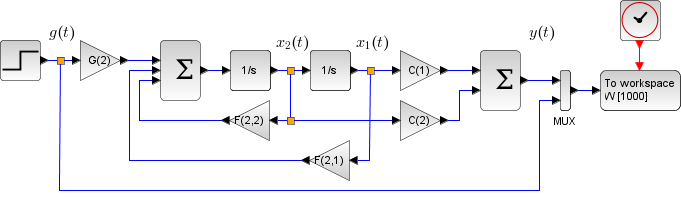
\includegraphics[width=1\textwidth]{mod_control.png}
	\caption{Схема моделирования замкнутой системы~\ref{eq_mod_control}}
	\label{fig:mod_control}
\end{figure}
\newpage


\begin{figure}[h]
	\centering
	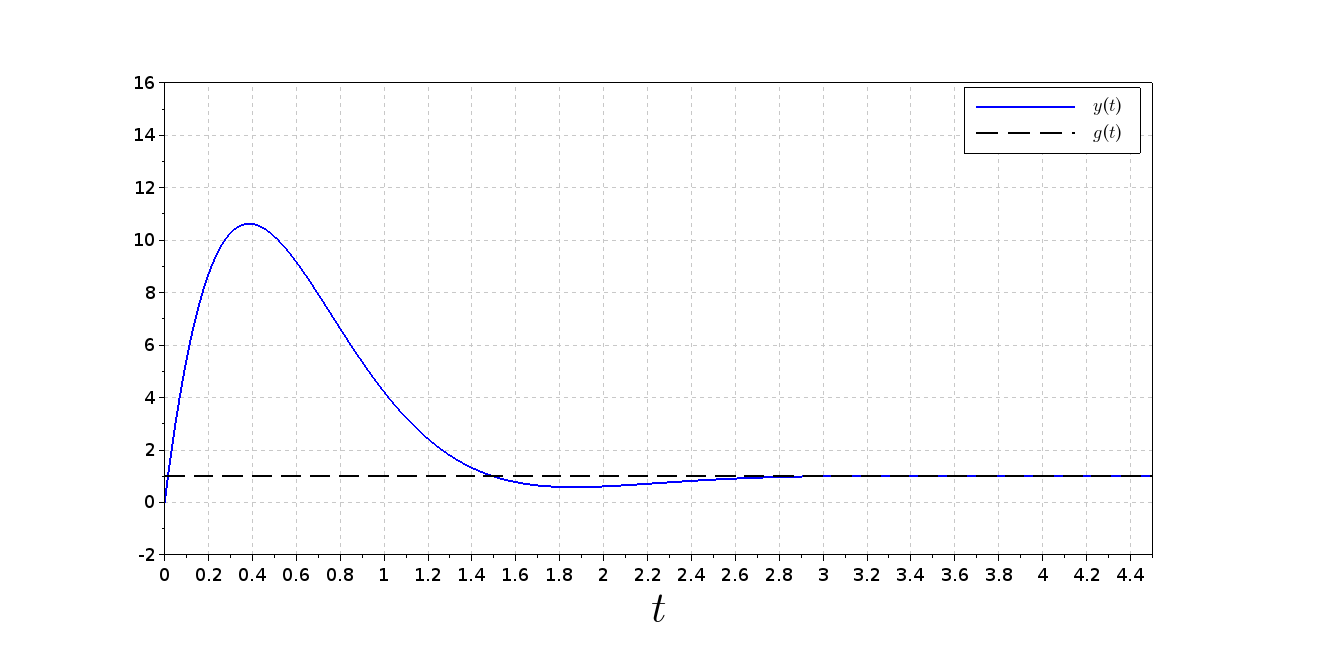
\includegraphics[width=1\textwidth]{res_mod_control.png}
	\caption{Переходная характеристика замкнутой системы~\ref{eq_mod_control}}
	\label{fig:mod_control}
\end{figure}

Таким образом, система обеспечивает равенство входа $g(t)$ и выхода $y(t)$ в неподвижном состоянии при номинальных значениях параметров $q_j$.

\subsection{Построение МТЧ спроектированной системы для каждого из параметров $q_j$}

Введем обозначения
\begin{align*}
&F_{q_j} = \cfrac{\partial{F(q)}}{\partial{q_j}} \bigg|_{q=q_0};
G_{q_j} = \cfrac{\partial{G(q)}}{\partial{q_j}} \bigg|_{q=q_0};
&F(q)|_{q=q_0} = F;
G(q)|_{q=q_0} = G;
\end{align*}

Подобно тому, как МТЧ строилась ранее, МТЧ замкнутой системы (ЗС)
\begin{equation}\label{eq_mts_ls_3}
	\begin{cases}
		\dot \sigma_j(t) &= F \sigma_j(t) + F_{q_j} x(t) + G_{q_j} g(t); 
		\sigma_j (0) = 0\\
		\eta_j (t) &= C \sigma_j (t) + C_{q_j} x(t)
	\end{cases}
\end{equation}

Пользуясь матрицами НОУ~\ref{Aq}~и~\ref{Bq}, рассчитаем матрицу $F(q) = A(q) - B(q) K$, где $K$~--- рассчитанная матрица коэффициентов ОС~\ref{Kq} (матрица $F(q)$ изображена транспонированной из соображений компактности записи)
\begin{equation}
	F(q) =
	\begin{bmatrix}
		0 & - \cfrac{(1+q_4)(1+q_7)}{2(1+q_3)(1+q_6)} - 8.5 \\
		1 & - \cfrac{20(1+q_3)(1+q_7)+3.6(1+q_4)(1+q_6)}{12(1+q_3)(1+q_6)} - 2.2753333
	\end{bmatrix}^T
\end{equation}

Рассчитаем матрицы для системы~\ref{eq_mts_ls_3} (матрицы $F_{q_j}$ приведены без операции транспонирования)

\begin{align}\label{mxs_sense}
&F_{q_{1,2}} = 
\begin{bmatrix}
0 & 0\\
0 & 0
\end{bmatrix};
F_{q_3} = 
\begin{bmatrix}
0 & 0\\
\cfrac{1}{2} & \cfrac{36}{120}
\end{bmatrix};
F_{q_4} = 
\begin{bmatrix}
0 & 0\\
- \cfrac{1}{2} & - 3.6
\end{bmatrix};
F_{q_6} = 
\begin{bmatrix}
0 & 0\\
\cfrac{1}{2} & \cfrac{20}{12}
\end{bmatrix};\\
&F_{q_7} = 
\begin{bmatrix}
0 & 0\\
- \cfrac{1}{2} & - \cfrac{20}{12}
\end{bmatrix};
G_{q_{1,2,3,4,6,7}} = 
\begin{bmatrix}
0\\
0
\end{bmatrix};
C_{q_1} = 
\begin{bmatrix}
0 & \cfrac{1}{4}
\end{bmatrix};
C_{q_2} = 
\begin{bmatrix}
\cfrac{1}{30} & 0
\end{bmatrix};\\
&C_{q_3} = 
\begin{bmatrix}
- \cfrac{1}{30} & - \cfrac{1}{4}
\end{bmatrix};
C_{q_4} = 
\begin{bmatrix}
0 & 0
\end{bmatrix};
C_{q_6} = 
\begin{bmatrix}
- \cfrac{1}{30} & - \cfrac{1}{4}
\end{bmatrix};
C_{q_7} = 
\begin{bmatrix}
0 & 0
\end{bmatrix};
\end{align}

Матрицы эквивалентны матрицам ОУ, так как матрица управления $B$ не зависит от параметров $q_j$.

Сконструируем агрегированную систему с составным вектором \newline $\tilde{x}_j=col\{x_j,\sigma_j\}$ размерности $ \dim \tilde{x} = 2n$, которая объединением \ref{eq_mod_control} и \ref{eq_mts_ls_3}, получает представление
\begin{align}\label{rang_system_3}
	\dot{\tilde{x}}_j (t) &= \tilde{F}_j \tilde{x}_j (t) + \tilde{G}_j g(t); 
	\tilde{x}_j (0) = col \{x(0), 0\}\\
	x(t) &= \tilde{C}_{x_j} \tilde{x}_j;\\
	y(t) &= \tilde{C}_j \tilde{x}_j (t);\\
	\sigma_j (t) &= \tilde{C}_{\sigma_j} \tilde{x}_j (t);\\
	\eta_j (t) &= \tilde{C}_{\eta_j} \tilde{x}_j (t)
\end{align}
где 
\begin{align*}
	&\tilde{{F}} =
	\begin{bmatrix}
	{F} & 0\\
	{F}_{q} & {F}
	\end{bmatrix},
	\tilde{{G}} = 
	\begin{bmatrix}
	{G}\\
	{G}_{q}
	\end{bmatrix},
\end{align*}

Структура матриц выхода $C$ совпадают с матрицами системы~\ref{rang_system}.
Составим матрицы агрегированной системы~\ref{rang_system_3}

\begin{align*}
	&\tilde{{F_{1,2}}} =
	\begin{bmatrix}
		  0   & 1     &  0  &  0\\     
		- 9 & - 4.242 &   0 &   0 \\    
		0   & 0  &     0  &  1     \\
		0   & 0 &    - 9 & - 4.242  	
	\end{bmatrix};
	\tilde{{F_3}} =
	\begin{bmatrix}
    0&     1&       0&    0.     \\
	- 9&   - 4.242 &  0&    0.    \\ 
	0&     0&       0&    1.    \\ 
	0.5 &  0.3 &  - 9&  - 4.242  
	\end{bmatrix};\\
	&\tilde{{F_4}} =
	\begin{bmatrix}
	    0&     1&       0&    0.     \\
		- 9&   - 4.242 &  0&    0.    \\ 
		0&     0&       0&    1.    \\ 
		-0.5 &  -0.3 &  - 9&  - 4.242  
	\end{bmatrix};
	\tilde{{F_6}} =
	\begin{bmatrix}
		0&     1&       0&    0.     \\
		- 9&   - 4.242 &  0&    0.    \\ 
		0&     0&       0&    1.    \\ 
		0.5  &  1.6666667 &  - 9&  - 4.242  
	\end{bmatrix};\\
	&\tilde{{F_7}} =
	\begin{bmatrix}
		0&     1&       0&    0.     \\
		- 9&   - 4.242 &  0&    0.    \\ 
		0&     0&       0&    1.    \\ 
		-0.5  &  -1.6666667 &  - 9&  - 4.242  
	\end{bmatrix};
	\tilde{{G}} =
	\begin{bmatrix}
		0\\1\\0\\0
	\end{bmatrix};\\
	&\tilde{{C}}_{\eta_1} =
	\begin{bmatrix}
		0&0.25&0.0333333 &   0.25\\
	\end{bmatrix}
	\tilde{{C}}_{\eta_2} =
	\begin{bmatrix}
		0.0333333&0&0.0333333 &   0.25\\
	\end{bmatrix}\\
	&\tilde{{C}}_{\eta_{3,7}} =
	\begin{bmatrix}
		-0.0333333&-0.25&0.0333333 &   0.25\\
	\end{bmatrix}
	\tilde{{C}}_{\eta_{4,7}} =
	\begin{bmatrix}
	0&0&0.0333333 &   0.25\\
	\end{bmatrix}
\end{align*}


Смоделируем полученную систему в пакете прикладных математических программ Scilab, подав в качестве входного сигнала единичное ступенчатое воздействие
\begin{figure}
	\centering
	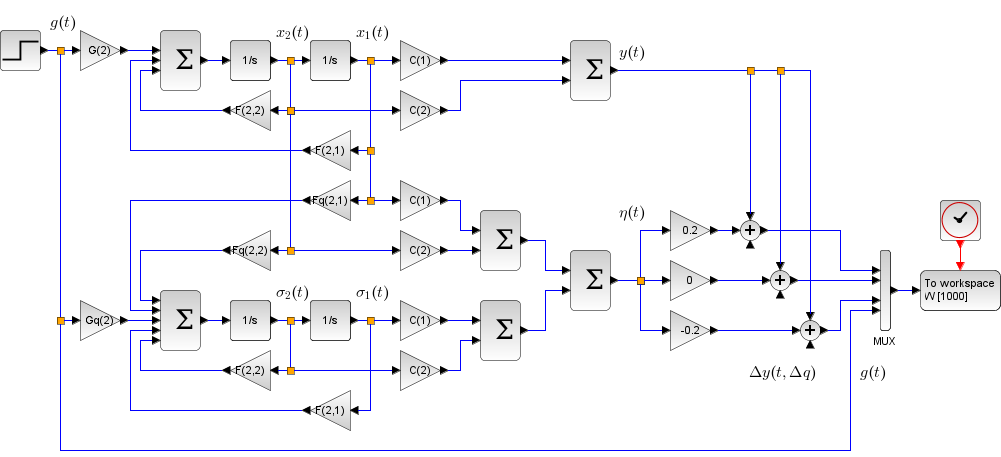
\includegraphics[width=1\textwidth]{mod_control_mts.png}
	\caption{Схема моделирования МТЧ дополненной НОУ~\ref{eq_mod_control}}
	\label{fig:mod_control_mts}
\end{figure}

\begin{figure}
	\centering
	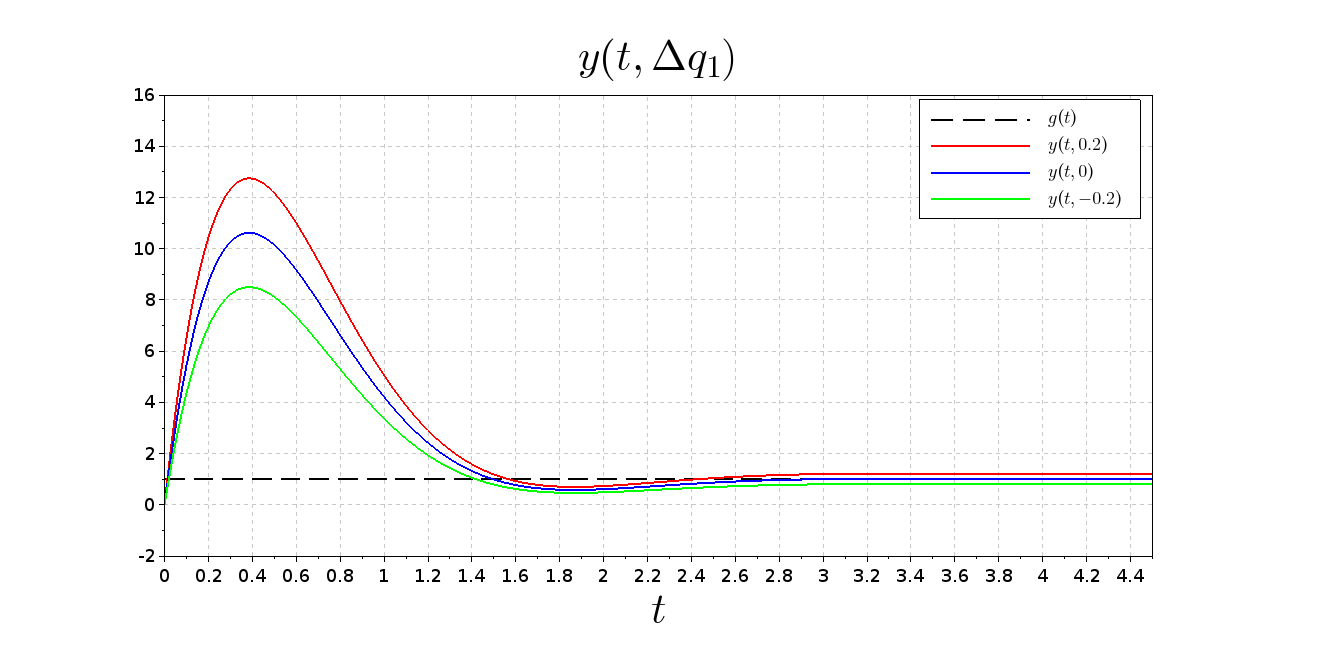
\includegraphics[width=1\textwidth]{res_3_q1.png}
	\caption{Переходные процессы при вариации параметра $q_1$}
	\label{fig:res_3_q1}
\end{figure}

\begin{figure}
	\centering
	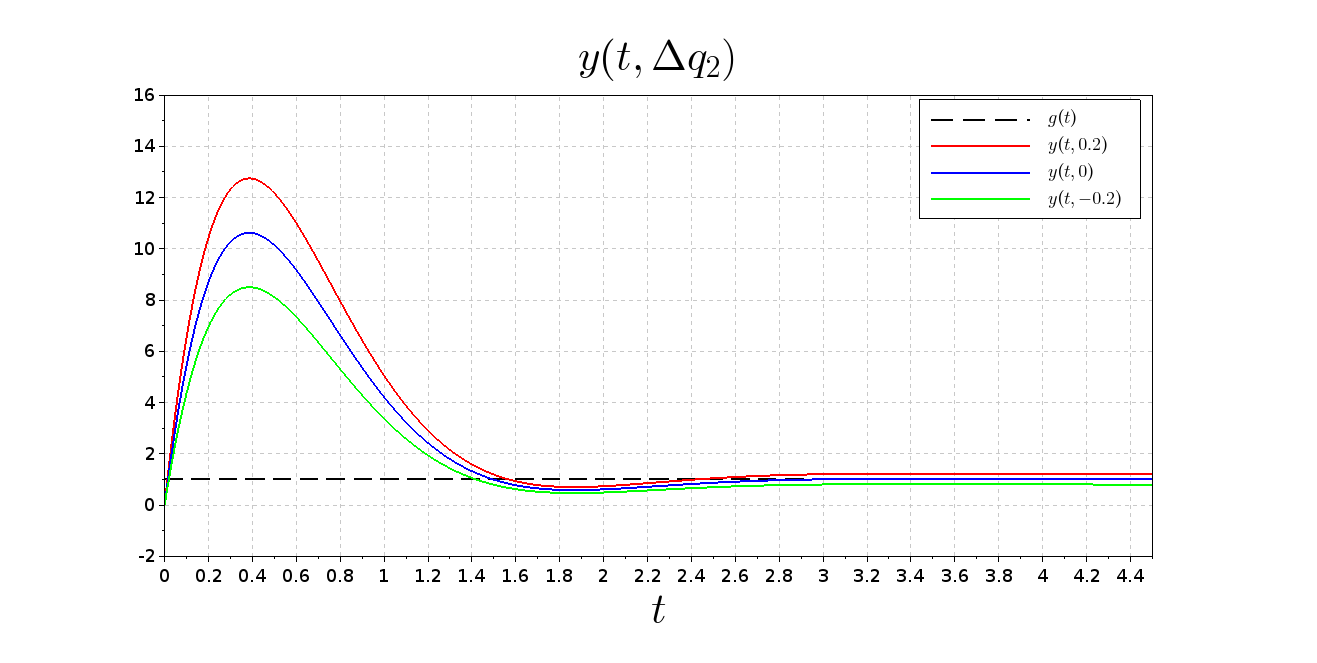
\includegraphics[width=1\textwidth]{res_3_q2.png}
	\caption{Переходные процессы при вариации параметра $q_2$}
	\label{fig:res_3_q2}
\end{figure}
\begin{figure}
	\centering
	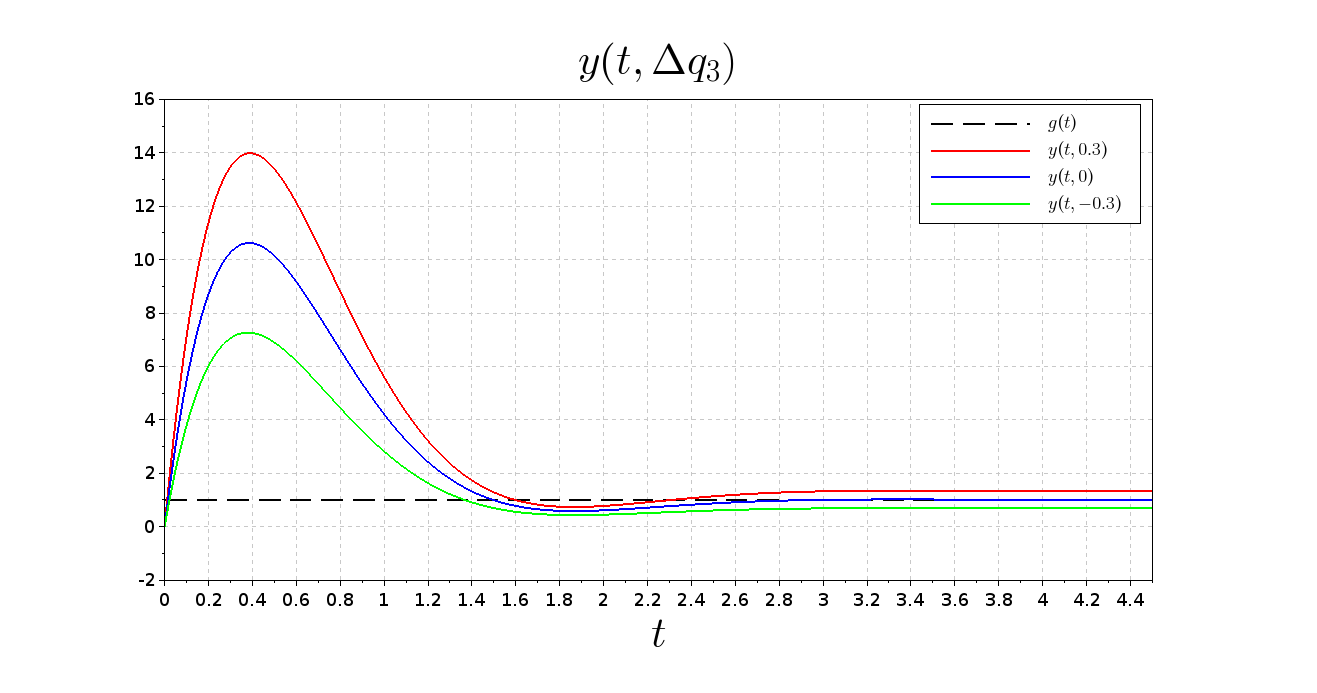
\includegraphics[width=1\textwidth]{res_3_q3.png}
	\caption{Переходные процессы при вариации параметра $q_3$}
	\label{fig:res_3_q3}
\end{figure}
\begin{figure}
	\centering
	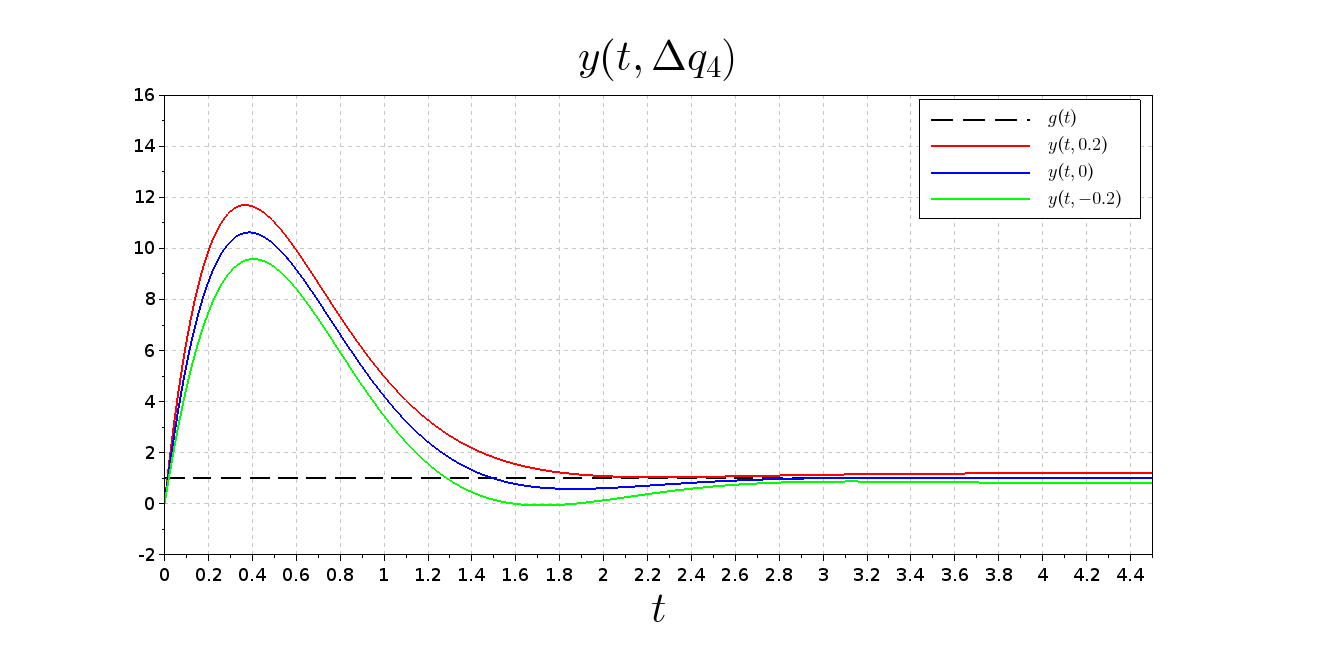
\includegraphics[width=1\textwidth]{res_3_q4.png}
	\caption{Переходные процессы при вариации параметра $q_4$}
	\label{fig:res_3_q4}
\end{figure}
\begin{figure}
	\centering
	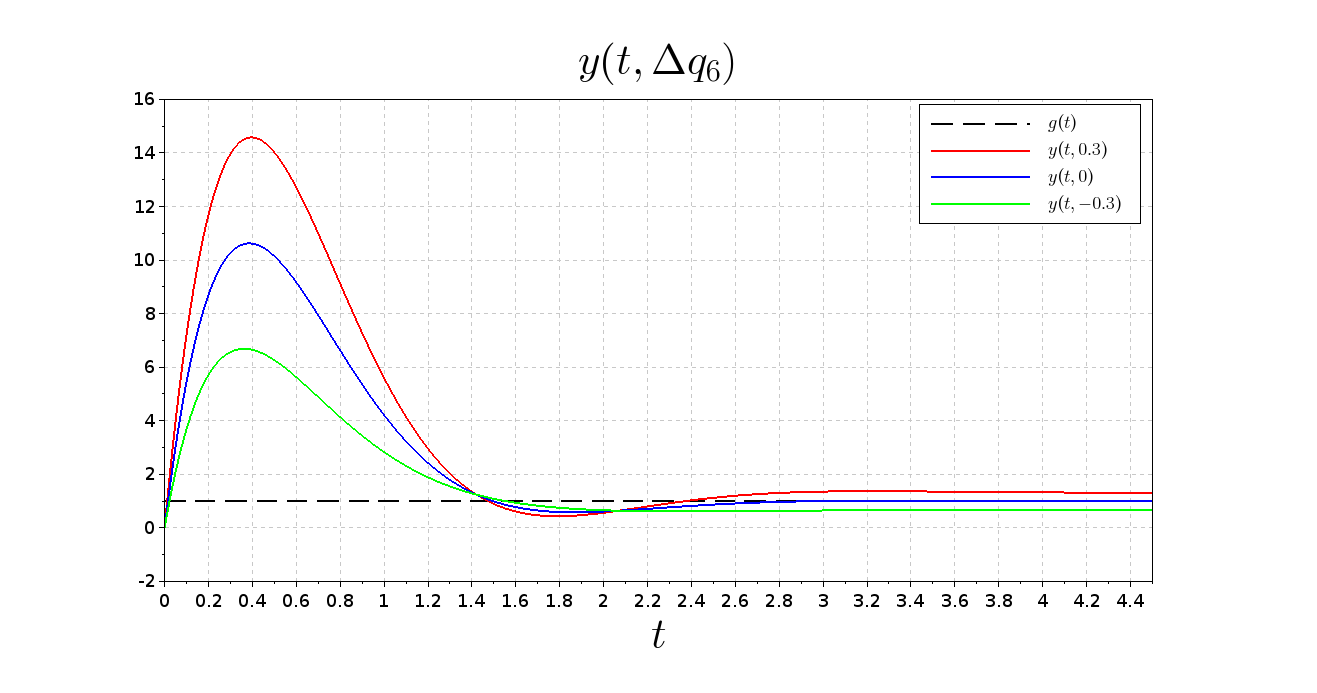
\includegraphics[width=1\textwidth]{res_3_q6.png}
	\caption{Переходные процессы при вариации параметра $q_6$}
	\label{fig:res_3_q6}
\end{figure}
\begin{figure}
	\centering
	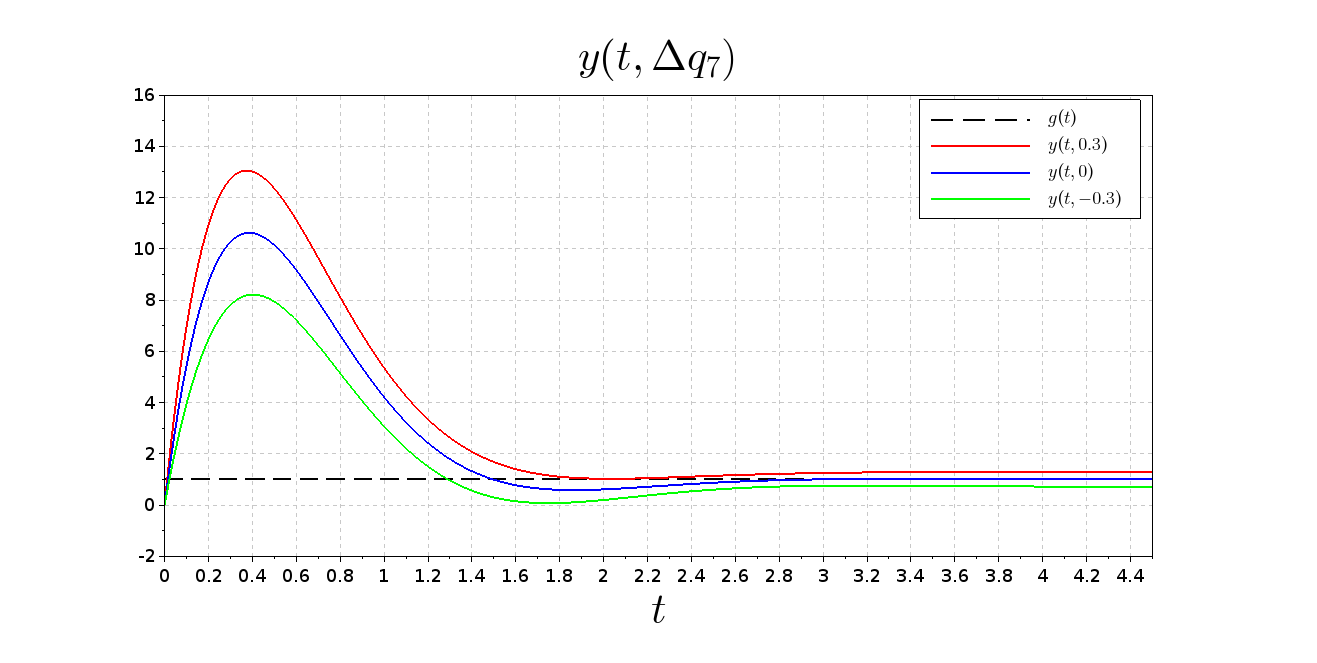
\includegraphics[width=1\textwidth]{res_3_q7.png}
	\caption{Переходные процессы при вариации параметра $q_7$}
	\label{fig:res_3_q7}
\end{figure}

\newpage
\subsection{Определение доминирующих параметров}

Занесем полученные из построенных графиков значения перерегулирования $\sigma$ и времени переходного процесса  $t_{\text{п}}$ в таблицу~\ref{t:dom}.

\begin{table}[h!]
	\centering
	\caption{Значения переререгулирования и времени преходного процесса для варьируемых парметров $q_j$}
	\label{t:dom}
	\begin{tabular}{|c|c|c|c|c|c|c|}
		\hline
		\multirow{2}{*}{Параметр} & \multicolumn{3}{c|}{\begin{tabular}[c]{@{}c@{}}Перерегулирование\\ $\sigma$, \%\\ при $\Delta q =$\end{tabular}} & \multicolumn{3}{c|}{\begin{tabular}[c]{@{}c@{}}Вр.перех.процесса\\ $t_\text{п}$, сек.\\ при $\Delta q =$\end{tabular}} \\ \cline{2-7} 
		& 0.2 & 0 & -0.2 & 0.2 & 0 & -0.2 \\ \hline
		$q_1$ & 1380 & \multirow{6}{*}{1062} & 745 & 2.72 & \multirow{6}{*}{2.72} & 2.72 \\ \cline{1-2} \cline{4-5} \cline{7-7} 
		$q_2$ & 1381 &  & 744 & 2.72 &  & 2.72 \\ \cline{1-2} \cline{4-5} \cline{7-7} 
		$q_3$ & 1398 &  & 727 & 2.69 &  & 2.81 \\ \cline{1-2} \cline{4-5} \cline{7-7} 
		$q_4$ & 1225 &  & 907 & 3.24 &  & 3.84 \\ \cline{1-2} \cline{4-5} \cline{7-7} 
		$q_6$ & 1458 &  & 669 & 3.37 &  & 3.26 \\ \cline{1-2} \cline{4-5} \cline{7-7} 
		$q_7$ & 1306 &  & 821 & 2.89 &  & 3.71 \\ \hline
	\end{tabular}
\end{table}

Рассчитаем отклонения значений перерегулирования $\Delta \sigma$ и времени переходного процесса $t_{\text{п}}$ характеристик системы при вариациях параметров $q_j$ от номинальной характеристики и занесем их в таблицу~\ref{t:res}.

\begin{table}[h!]
	\centering
	\caption{Отклонения характеристик системы с варьируемыми параметрами от номинальной системы}
	\label{t:res}
	\begin{tabular}{|c|c|c|c|c|}
		\hline
		\multirow{2}{*}{Параметр} & \multicolumn{2}{c|}{\begin{tabular}[c]{@{}c@{}}$\Delta \sigma$, \%\\ при $\Delta q = $\end{tabular}} & \multicolumn{2}{c|}{\begin{tabular}[c]{@{}c@{}}$\Delta t_\text{п}$, сек.\\ при $\Delta q = $\end{tabular}} \\ \cline{2-5} 
		& 0.2 & -0.2 & 0.2 & -0.2 \\ \hline
		$q_1$ & 318 & 317 & 0    & 0 \\ \hline
		$q_2$ & 318 & 319 & 0 & 0 \\ \hline
		$q_3$ & 336 & 335 & 0.03 & 0.09 \\ \hline
		$q_4$ & 163 & 155 & 0.52 & 1.12 \\ \hline
		$q_6$ & 396 & 393 & 0.65 & 0.54\\ \hline
		$q_7$ & 244 & 241 & 0.17& 0.99 \\ \hline
	\end{tabular}
\end{table}
где
\begin{equation}
	\Delta \sigma_{\Delta q = \pm 0.2} = |\sigma_{\Delta q = \pm 0.2} - \sigma_{\Delta q = 0}|
\end{equation}

\begin{equation}
	\Delta t_{\text{п}, \Delta q = \pm 0.2} = |t_{\text{п}, \Delta q = \pm 0.2} - t_{\text{п}, \Delta q = 0}|
\end{equation}

Выделим доминирующие параметры по степени их влияния на величину $\sigma$ перерегулирования и длительности $t_\text{п}$ переходного процесса

	
\begin{enumerate}
	\item Влияние на величину перерегулирования (в порядке уменьшения)
		\begin{enumerate}
			\item при $\Delta q = 0.2$: 
				$q_6$,
				$q_3$,
				$q_2$,
				$q_1$,
				$q_7$,
				$q_4$;					
			\item при $\Delta q = -0.2$
				$q_6$,
				$q_3$,
				$q_2$,
				$q_1$,
				$q_7$,
				$q_4$;					
		\end{enumerate}	
	\item Влияние на время переходного процесса(в порядке уменьшения)
		\begin{enumerate}
			\item при $\Delta q = 0.2$: 
			$q_6$,
			$q_5$,
			$q_7$,
			$q_3$,
			$q_{1,2}$;
			\item при $\Delta q = - 0.2$: 
			$q_4$,
			$q_7$,
			$q_6$,
			$q_3$,
			$q_{1,2}$.
		\end{enumerate}	
\end{enumerate}

\newpage
\section{Построение МФМЧ и результаты ее исследования}

\begin{enumerate}
	\item Построить матрицу функций модальной чувствительности;
	\item Выделить неблагоприятное сочетание вариаций параметров.
\end{enumerate}

\subsection{Построение МФМЧ}

Для вычисления функций чувствительности $\delta q_j$ и $\beta q_j$ соответственно вещественных и мнимых частей комплексно-сопряженных собственных значений к вариациям параметра $q_j$ следует вычислить матрицу $M^{-1} F_{q_j} M$ и на элементах этой матрицы сконструировать функции чувствительности $\delta q_j$ и $\beta q_j$ с помощью соотношений
\begin{align}\label{fsenses}
	\delta_{q_j} = \cfrac{1}{2} \left( (M^{-1} F_{q_j} M)_{11} + (M^{-1} F_{q_j} M)_{22}\right)\\
	\beta_{q_j} = \cfrac{1}{2} \left((M^{-1} F_{q_j} M)_{12} - (M^{-1} F_{q_j} M)_{21} \right)
\end{align}
где матрица $M$~--- матрица диагонального преобразования, $F_{q_j}$~--- матрица чувствительности замкнутой системы к вариации параметра $q_j$.

Найдем спектр собственных значений матрицы $F(q)$ при номинальном векторе параметров $q$
\begin{equation}
	\sigma{\{F\}} = \{[\lambda_1, \lambda_2] :det[\lambda I - F] = 0\} = \{- 2.121 \pm j 2.1216406 \}
\end{equation}

Для анализа модальной чувствительности спроектированной системы произведем следующие вычисления. Матрицы чувствительности $F_{q_j}$ были рассчитаны ранее в ~\ref{mxs_sense}.

Матрица $M$ находится из выражения
\begin{equation}
	M \Lambda = F M
\end{equation}

Так как в спектре $\sigma{\{F\}}$ имеются комплексно-сопряженные собственные значения $\lambda_{1,2} = \delta \pm j \beta$, то вещественная матрица подобия $\Lambda$ будет блочно-диагональной 
\begin{equation}
	\Lambda = 
	\begin{bmatrix}
		\delta &  \beta\\
		-\beta & \delta
	\end{bmatrix}
	=
	\begin{bmatrix}
	  - 2.121  &      2.1216406  \\
		-2.1216406&  - 2.121 
	\end{bmatrix}
\end{equation}


Тогда, нужно записать матрицу $M$ в форме обобщенной матрицы Вандермонда
\begin{equation}
	M = 
	\begin{bmatrix}
	1&0\\
	\delta&\beta
	\end{bmatrix}
	=
	\begin{bmatrix}
	1&0\\
	-2.121&  2.1216406 
	\end{bmatrix}
\end{equation}

Матрица $M^{-1}$
\begin{equation}
	M^{-1} = 
	\begin{bmatrix}
	   1&           0\\         
	0.9997105  &  0.4519487 
	\end{bmatrix}
\end{equation}

Вычислим матрицы $(M^{-1} F_{q_j} M)$, при $j = \overline{1,2,3,4,6,7}$
\begin{equation}
	M^{-1} F_{q_{1,2}} M = 
	\begin{bmatrix}
	0&0\\
	0&0	
	\end{bmatrix}
\end{equation}
\begin{equation}
	M^{-1} F_{q_3} M = 
	\begin{bmatrix}
	    0&           0\\   
	- 0.0739388  &  0.3 	
	\end{bmatrix}
\end{equation}
\begin{equation}
	M^{-1} F_{q_4} M = 
	\begin{bmatrix}
	    0&           0\\   
	3.3729834 & - 3.6
	\end{bmatrix}
\end{equation}
\begin{equation}
	M^{-1} F_{q_6} M = 
	\begin{bmatrix}
	    0&           0\\         
	- 1.4402098&    1.6666667 
	\end{bmatrix}
\end{equation}
\begin{equation}
	M^{-1} F_{q_7} M = 
	\begin{bmatrix}
    0&           0\\         
	1.4402098 & - 1.6666667 	
	\end{bmatrix}
\end{equation}

В соответствии с выражениями~\ref{fsenses}, вычислим функции модальной чувствительности $\lambda_{q_j} = \delta_{q_j} \pm j \beta_{q_j}$
\begin{equation}
	\lambda_{q_{1,2}} = 0
\end{equation}
\begin{equation}
\lambda_{q_3} = 0.15 + j 0.0369694 
\end{equation}
\begin{equation}
\lambda_{q_4} =  - 1.8 - j  1.6864917 
\end{equation}
\begin{equation}
\lambda_{q_6} = 0.8333333 + j 0.7201049 
\end{equation}
\begin{equation}
\lambda_{q_7} = - 0.8333333  - j 0.7201049  
\end{equation}

Сконструируем матрицу функций модальной чувствительности в виде функций чувствительности вещественной и мнимой частей:
\begin{equation}
	S_{\lambda} = 
	\begin{bmatrix}
	\delta_q\\
	\beta_q
	\end{bmatrix}
	=
	\begin{bmatrix}
	0&0& 0.15 &- 1.8  & 0.8333333 &  - 0.8333333\\
	0&0& 0.0369694 &-1.6864917&  0.7201049 & -0.7201049  
	\end{bmatrix}
\end{equation}

\subsection{Выделить неблагоприятное сочетание вариаций параметров}

Для выделения неблагоприятного сочетания вариаций параметров воспользуемся сингулярным разложением матрицы модальной чувствительности
\small
\begin{align*}
	&S_{\lambda} = U_{\lambda} \Sigma_{\lambda} V^T_{\lambda}\\
	&U_{\lambda} = \begin{bmatrix}
	  - 0.7383 & - 0.6744  \\
	- 0.6744  &  0.7383 
	\end{bmatrix}\\
	&\Sigma_{\lambda} = 
	\begin{bmatrix}
	    2.9199   & 0  &         0&    0&    0&    0\\  
		0&           0.0909   & 0&    0&    0&    0 
	\end{bmatrix}\\
	&V_{\lambda} =
	\begin{bmatrix}
	0 & 0 &   0.0695&  - 0.8346    &0.3863&  - 0.3863  \\
	0         &  0         &- 0.8105  &- 0.3666234  &- 0.3230   & 0.3230  \\
	- 0.0464 & - 0.8121 &   0.3382&  - 0.2391&  - 0.2886&    0.2886\\  
	0.8446 & - 0.3427 & - 0.2391   & 0.169  &  0.204  &- 0.204  \\
	- 0.377 & - 0.3338 & - 0.2886 &   0.204 &   0.7463 &   0.2536  \\
	0.377   & 0.3338    &0.2886  &- 0.204   & 0.2536    &0.7463 	
	\end{bmatrix}
\end{align*}
\normalsize
%Выделим согласованные тройки $\{U_{\lambda max}, \alpha_{\lambda max}\}, V_{\lambda max}\}$ и \newline
%$\{U_{\lambda min}, \alpha_{\lambda min}\}, V_{\lambda min}\}$, то на фиксированной в %сфере $||\Delta q|| = 0.2$ в пространстве параметров могут быть получены оценки
%\begin{equation}
%	\max_{\Delta q} ||\Delta \lambda|| = \alpha_{\lambda M} ||\Delta q||
%\end{equation}
%\begin{equation}
%	\min_{\Delta q} ||\Delta \lambda|| = \alpha_{\lambda m} ||\Delta q||
%\end{equation}
%максимальной и минимальной по норме вариации собственных значений, при этом правые ингулярные векторы $V_{\lambda max}$ и $V_{\lambda min}$ задают наиболее неблагоприятное и наименее неблагоприятное сочетание параметров, порождающих соответственно вариации.

Запишем оценки вариации
\begin{equation}
\max_{\Delta q} ||\Delta \lambda|| =  2.9199 ||\Delta q||
\end{equation}
\begin{equation}
\min_{\Delta q} ||\Delta \lambda|| = 0.0909 ||\Delta q||
\end{equation}

Наиболее неблагоприятное сочетание вариаций параметров характеризуется вектором
\begin{equation}
	\Delta q = 
	\begin{bmatrix}
	0&0&- 0.0464681 &   0.8446960 & - 0.3770473 &   0.3770473 
	\end{bmatrix}^T
	||\Delta q||
\end{equation}

Наименее неблагоприятное характеризуется вектором
\begin{equation}
	\Delta q = 
	\begin{bmatrix}
		0&0&  - 0.8121559 & - 0.3427354 & - 0.3338676  &  0.3338676 
	\end{bmatrix}
	||\Delta q||
\end{equation}


\newpage
\section{Получение ВМО НОУ с интервальными параметрами}

\begin{enumerate}
	\item Получение ВМО НОУ с интервальными параметрами
	\begin{equation}\label{VMO}
		\begin{cases}
			\dot x (t)  = [A] x(t) + [B] u(t);\\
			y(t) = C x(t)			
		\end{cases}
	\end{equation}
	где $[A] = A_0 + [\Delta A], [B] = B_0 + [\Delta B]$
	c использованием интервальной арифметики на основе интервальной реализации параметров $q_j$, записываемых в форме $[q_j] = [\underline{q_j}, \overline{q_j}]$ при заданных граничных (угловых) значениях.
\end{enumerate}

\subsection{Построение векторно-матричное описание НОУ}



\newpage
\section{Построение медианного МУ НОУ и оценка его результатов}

\begin{enumerate}
	\item *Представить ОУ~\ref{eq_iso_coc} в базисе, в котором 	неопределенность физических параметров представлена 	неопределенностью значений только матрицы состояния в	форме матричного компонента $\Delta A$;  
	\item Синтезировать закон медианного модального управления, базовый алгоритм которого дополняется контролем нормы  медианной составляющей интервальной матрицы  спроектированной системы с последующим вычислением оценки, вычислить матрицы $K_g$ и $K$. 
	Закон управления (ЗУ) вида $u(t) = K_g g(t)-K x(t)$ должен доставлять системе
	\begin{equation}
		\begin{cases}
			\dot x (t) = [F] x(t) + G g(t);\\
			y(t) = C x(t)
		\end{cases}
	\end{equation}
	образованной объединением НОУ и ЗУ равенство входа $g(t)$ и выхода $y(t)$ в неподвижном состоянии при номинальных значениях параметров с помощью:
	\begin{enumerate}
		\item матрицы $K_g$ прямой связи по входу $g(t)$;
		\item матрыцы $K$ обратной связи по состоянию $x(t)$
	\end{enumerate}
	распределение мод Баттерворта с характеристической частотой $\omega_0 = 3c^{-1}$, которая гарантирует достижение значение оценки относительной интервальности матрицы состояния системы $\delta_I = \cfrac{||\Delta F||}{||F_0||}$ не больше заданной $\delta_{IR}F = 0.02$; 
	\item Исследовать свойство робастности системы, полученной в п.1, с помощью метода В.Л. Харитонова;
	\item Моделирование полученной системы.
\end{enumerate}

\subsection{Получение ВМО НОУ с интервальными параметрами только матрицы состояния}

Модельная параметрическая неопределенность может быть представлена неопределенностью (интервальностью) задания только матрицы состояния объекта управления. Таким образом, объект управления с интервальными параметрами задается векторно-матричной моделью
\begin{equation}\label{eq:mmc}
	\begin{cases}
		\dot x (t) = [A] x(t) + B u(t);\\
		y(t) = C x(t)
	\end{cases}
\end{equation}
где $x \in R^n, u \in R^r, y \in R^m$ -- соответственно векторы состояния, управления и выхода ОУ; $[A], B, C$ -- интервальная матрица состояния, матрица управления и выхода, согласованные по размерности с переменными модели~\ref{eq:mmc}.

Из предыдущего утверждения становится очевидным, что матрицы ОУ полученные в п.5 не соответствуют предъявляемым к ним требованиям и нужно представить ОУ в форме~\ref{eq:mmc}.

Для этого нужно ОУ~\ref{eq_OU} привести к наблюдаемой (фробениусовой) канонической форме, тогда его матрицы примут вид
\begin{equation}\label{Aqn}
	A(q) =
	\begin{bmatrix}
	0 & - \cfrac{(1+q_4)(1+q_7)}{2(1+q_3)(1+q_6)} \\
	1 &-\cfrac{20(1+q_3)(1+q_7)+3.6(1+q_4)(1+q_6)}{12(1+q_3)(1+q_6)}
	\end{bmatrix}
\end{equation}
\begin{equation}\label{Bqn}
	B(q) =
	\begin{bmatrix}
		\cfrac{(1 + q_2)}{30(1+q_3)(1+q_6)}\\
		\cfrac{(1 + q_1)}{4(1+q_3)(1+q_6)} 
	\end{bmatrix}
\end{equation}

\begin{equation}\label{Cqn}
	C =
	\begin{bmatrix}
	0 & 1
	\end{bmatrix}
\end{equation}

Затем, так как полученные ОУ в каноническом наблюдаемом базисе не позволяет параметрическую неопределенность представить только в виде вариации $\Delta A$ матрицы
состояния, то на входе ОУ достаточно включить буферную систему~\cite{NSUsh}
\begin{equation}
	\begin{cases}
		{\dot x_B} (t) = A_B x_B(t) + B_B u_B(t) u(t);\\
		y(t) = C_B x_B(t)
	\end{cases}
\end{equation}
минимальной размерности $\dim x_B = \dim u = r = 1$ и ввести в рассмотрение составной вектор $\tilde{x} = col\{x, x_B\}$ и $\tilde{u} = col\{u, u_B\}$, получим систему
\begin{equation}
	\begin{cases}
		\tilde{\dot x} (t) = \tilde{A} \tilde{x}(t) + \tilde{B} \tilde{u}(t);\\
		y(t) = \tilde{C} \tilde{x}(t)
	\end{cases}
\end{equation}
где
\begin{align}
	\tilde{A} =
	\begin{bmatrix}
	 A(q) & B(q) C_B\\
	 0 & A_B
	\end{bmatrix};
	\tilde{B} = 
	\begin{bmatrix}
		0\\
		B_B
	\end{bmatrix};
	\tilde{C} = 
	\begin{bmatrix}
		C & 0
	\end{bmatrix}
\end{align}

Составим матрицы, при $A_B = 0, B_B = 1, C_B = 1$
\begin{align}
	\tilde{A} =&
	\begin{bmatrix}
		0 & - \cfrac{(1+q_4)(1+q_7)}{2(1+q_3)(1+q_6)} &	\cfrac{(1 + q_2)}{30(1+q_3)(1+q_6)}\\
		1 &-\cfrac{20(1+q_3)(1+q_7)+3.6(1+q_4)(1+q_6)}{12(1+q_3)(1+q_6)} & \cfrac{(1 + q_1)}{4(1+q_3)(1+q_6)} \\
		0&0&0
	\end{bmatrix};\\
	\tilde{B} =&
	\begin{bmatrix}
	0\\
	0\\
	1
	\end{bmatrix};
	\tilde{C} =
	\begin{bmatrix}
	0 & 1 & 0
	\end{bmatrix}
\end{align}

В соответствии с~\ref{interv},~\ref{midA},~\ref{widA}, запишем интервальную матрицу $[\tilde{A}] = \tilde{A}_0 + [\Delta A]$
\begin{align}
	[\tilde{A}] =
	\begin{bmatrix}
	    0&  - 0.6736111 &   0.0405093  \\
		1&  - 2.649537  &   0.3038194  \\
		0&    0        & 0 
	\end{bmatrix}
	+
	\begin{bmatrix}
		0&	[- 0.4514, 0.4514]	&[-0.02199, 0.02199] \\
		0&	[-1.7755, 1.7755]	&[-0.1649, 0.1649]\\
		0&0&0
	\end{bmatrix}
\end{align}

Таким образом, ОУ~\ref{eq:mmc} характеризуется параметрической неопределенностью только матрицы состояния.


\subsection{Синтез медианного МУ НОУ}

Порядок полученного в пункте 6.1 ОУ $\dim n = 3$, а ранг матрицы $\tilde{B}$ $rang \tilde{B} = 2$ и $rang \tilde{B} < \dim n$, следовательно возможно решение только неполной задачи обобщенного модального управления (ОМУ).

Агрегирование полученного ОУ и ЗУ
\begin{equation}
	u (t) = K_g g(t) - K x(t)
\end{equation}
образует систему 
\begin{equation}
	\begin{cases}
		\dot x (t) = [F] x(t) + G g(t);\\
		y(t) = C x(t)
	\end{cases}
\end{equation}
где 
\begin{equation}
	[F] = F_0 + \Delta F, \Delta F = \Delta A, G = B K_g.
\end{equation}

Найдем нормы медианной и интервальной составляющих матрицы $\tilde{A}$ (далее будем ее обозначать как $A$)
\begin{align}
    ||A_0|| = 2.92; ||\Delta A|| = 1.84
\end{align}

%Сформируем требования к показателям качества проектируемой системы: пусть $t_{n} \le 20c,  \sigma \le 50\%, \delta_{IR} F = 0.02$.

Выберем наблюдаемую пару матрицу модальной модели ($\Lambda$, H). Назначим матрицу $\Lambda$, соответствующую круговому распределению мод с характеристической частотой $\omega_0$ такой, что $||\Lambda|| \ge \omega_0$ и
\begin{equation}
	\Lambda = \arg\{||\Lambda|| \ge \cfrac{||\Delta A||}{\delta_{I} F} \& \sigma\{\Lambda\} = \sigma\{F\} \}
\end{equation}

Значение характеристической частоты $\omega_0$ определяется в силу технических требований к проектируемой системе из условия
\begin{equation}
	\omega_0 = max \{\omega_0 <= \cfrac{6}{2} = 3c^{-1}; \omega_0 <= \cfrac{||\Delta A||}{\delta_{IR}} = \cfrac{2.92}{0.02} =  146c^{-1}\} = 146 c^{-1}
\end{equation}

Найдем матрицу $\Lambda$
\begin{align}
	\Lambda = \omega_0 
	\begin{bmatrix}
	  - 0.0260481&    0.   &        0.\\         
		0.    &     - 0.0011358 &   0.  \\       
		0.   &        0.      &   - 12.057286 	
	\end{bmatrix}
	=\\=
	\begin{bmatrix}
	  - 3.8030252   & 0.       &    0.\\         
		0.        & - 0.1658288&    0.  \\       
		0.        &   0.    &     - 1760.3637 
	\end{bmatrix}
\end{align}
\begin{equation}
	||\Lambda|| = 1760.36
\end{equation}

Модификация матрицы $H$ осуществляется в силу алгоритмов линейного программирования,
таких как алгоритм Нелдера–Мида. В итоге матрица $M$ ищется с помощью итерационной процедуры, приводящей к выполнению условия:
\begin{equation}
	M = \arg \min_H \{C\{M(H)\} : M \Lambda - A M = - B H : \Lambda = fix, H = var\}
\end{equation}
где начальное значение $H = \begin{bmatrix}1&1&1\end{bmatrix}$.

Выполнение этой процедуры дает следующие реализации матриц 
\begin{equation}
	H = 
	\begin{bmatrix}
	 - 0.0053596  &  0.000099  &  2.3063721 
	\end{bmatrix}
\end{equation}
\begin{equation}
	M = 
	\begin{bmatrix}
	    0.00007 &  - 0.0002374 & - 3.024D-08\\  
		0.0003105 & - 0.0000225 & - 0.0000002 \\ 
		- 0.0014093 &   0.0005972 &   0.0013102 
	\end{bmatrix}
\end{equation}

Наименьшее число обусловленностей, которой удалось получить при задании различных комбинация матриц $\Lambda$
\begin{equation}
	C\{M\} = 9.45
\end{equation}

Произведем расчет матриц регулятора. Матрицы ОС $K$ имеет реализацию
\begin{equation}
	K = H M^{-1} = 
	\begin{bmatrix}
	3754.6837 &   7131.9983   & 1761.6831
	\end{bmatrix}
\end{equation}

Матрица прямых связей $K_g$
\begin{equation}
	K_g = -(C * F^(-1) * B)^(-1) =
	\begin{bmatrix}
		27422.098 
	\end{bmatrix}
\end{equation}

Вычислим матрицу замкнутой системы $F$ 
\begin{equation}
	F0 = A0 - B K =
	\begin{bmatrix}
	    0.&        - 0.6736111 &   0.0405093  \\
		1. &        - 2.649537  &   0.3038194  \\
		- 3754.6837 & - 7131.9983 & - 1762.6831 
	\end{bmatrix}
\end{equation}

Вычислим полученную оценку относительной интервальности матрицы~$F$
\begin{equation}
	\delta_{IF} = \cfrac{||\Delta A||}{||F0||} = \cfrac{1.84}{8250.46} = 0.0002229 < 0.02
\end{equation}

\subsection{Исследование свойства робастности системы}
Представим матрицу $F$ в интервальном виде
\begin{equation}
	\Delta F = \Delta A = 
	\begin{bmatrix}
		0  &[- 0.45138, 0.45138] &  [- 0.02199, 0.02199]\\  
		0  &[- 1.7754, 1.7754] &   [- 0.16493, 0.16493]  \\
		0  &  0     &      0         
	\end{bmatrix}
\end{equation}


\begin{equation}
	[F] = 
	\begin{bmatrix}
	0 &        [- 1.125, - 0.2222222] &       [0.0185185, 0.0625]  \\ 
	1  &       [- 4.425, - 0.8740741]  &      [0.1388889, 0.46875]  \\
	- 3754.6837 & - 7131.9983&  - 1762.6831  

	\end{bmatrix}
\end{equation}

Найдем характеристический полином $D(\lambda, q)$ матрицы $F(q)$
\begin{equation}\label{char}
	D(\lambda, q) = det(\lambda I -F(q)) = [a_0] \lambda^3 + [a_1] \lambda^2 + [a_2] \lambda + [a_3]
\end{equation}
где $[a_n]$~-- интервальный параметр вида $[\underline{a_n}, \overline{a_n}]$.

По теореме В. Л. Харитонова, чтобы интервальный характеристический полином~\ref{char}
был гурвицевым необходимо и достаточно, чтобы были гурвицевыми четыре его угловые версии, имеющие представления
\begin{align}
	&D(\lambda) = \underline{a_3} + \underline{a_2} \lambda + \overline{a_1} \lambda^2 + \overline{a_0} \lambda^3\\
	&D(\lambda) = \overline{a_3} + \underline{a_2} \lambda + \underline{a_1} \lambda^2 + \overline{a_0} \lambda^3\\
	&D(\lambda) = \overline{a_3} + \overline{a_2} \lambda + \underline{a_1} \lambda^2 + \underline{a_0} \lambda^3\\
	&D(\lambda) = \underline{a_3} + \overline{a_2} \lambda + \overline{a_1} \lambda^2 + \underline{a_0} \lambda^3
\end{align}

Найдем интервальные коэффициенты ИХП~\ref{char} методом Крамера
\begin{align}
	&[a_0] = [1,1];\\
	&[a_1] = -tr[F] = [178579.4658, 178583.0167];\\
	&[a_2] = [M_{11}] + [M_{22}] = [136062041.6772, 136697531.9607];\\
	&[a_3] = -det[F] = [43933256.2435, 156394735.1753]
\end{align}

Тогда полиномы запишутся, как 
\begin{align}
	&D(\lambda) = 43933256.2435 + 136062041.6772 \lambda + 178583.0167 \lambda^2 + \lambda^3\\
	&D(\lambda) = 156394735.1753 + 136062041.6772 \lambda + 178579.4658 \lambda^2 + \lambda^3\\
	&D(\lambda) = 156394735.1753 + 136697531.9607 \lambda + 178579.4658 \lambda^2 + \lambda^3\\
	&D(\lambda) = 43933256.2435 + 136697531.9607 \lambda + 178583.0167 \lambda^2 + \lambda^3
\end{align}

Все полиномы В. Л. Харитонова гурвицевы, следовательно, гурвицев ИХП $[D(\lambda)]$. Система робастно устойчива.

\subsection{Моделирование полученной системы}

\begin{figure}[h!]
	\centering
	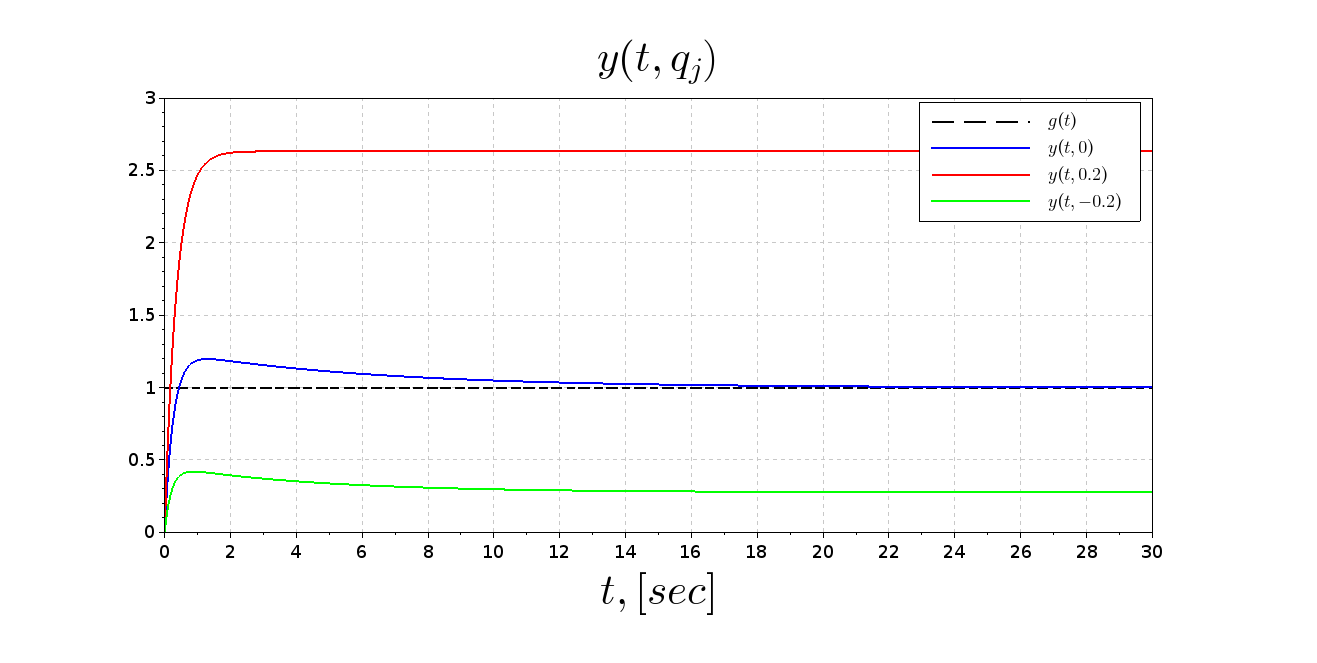
\includegraphics[width=1\textwidth]{problem6_res.png}
	\caption{Результаты моделирования ММУ при $q = [\underline{-0.2}, \overline{0.2}]$}
	\label{}
\end{figure}
\newpage



\begin{figure}[h!]
	\centering
	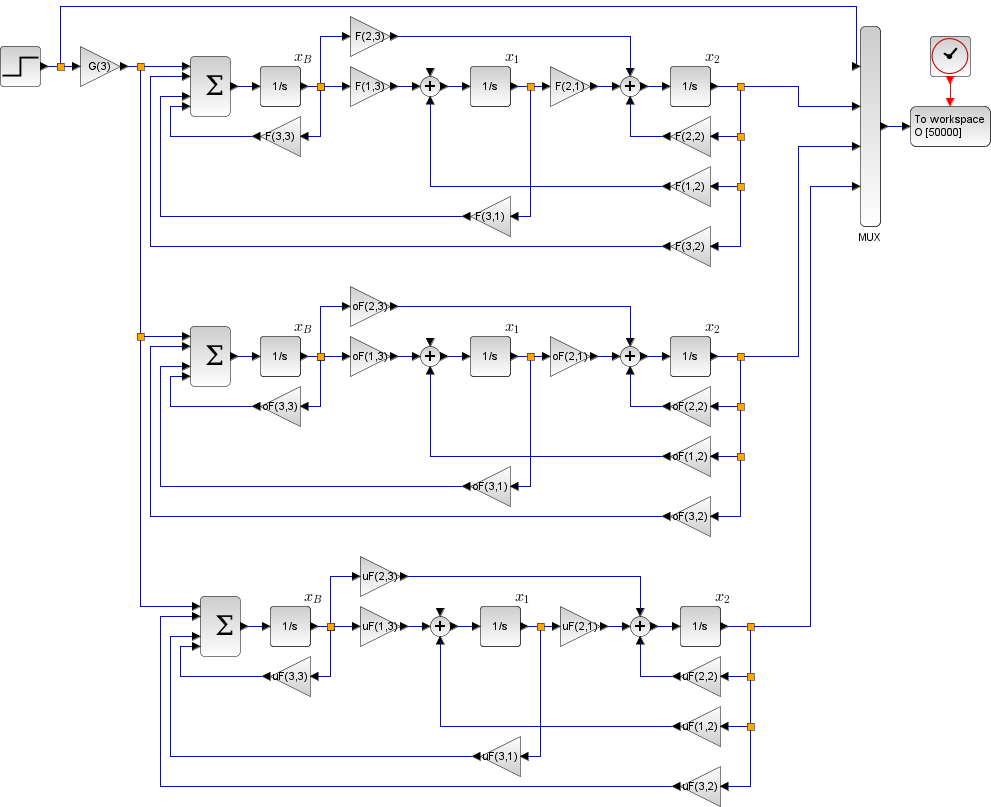
\includegraphics[width=1\textwidth]{problem6.png}
	\caption{Схема моделирования ММУ}
	\label{}
\end{figure}


\newpage
%\section*{Заключение}
\addcontentsline{toc}{section}{Заключение}
Текст заключения
\newpage
\renewcommand\refname{Список использованных источников}
\providecommand*{\url}[1]{#1} %нужно для описания некоторых источников
\bibliography{used_books}
%\ESKDappendix{обязательное}{Название приложения}\label{append_app_example}
Текст приложения
\end{document}